\subsubsection*{Project 1: Investigate structural modifications of irradiated silica for nuclear materials}\label{lang}

The first project would be the study of the local structure changes in amorphous silica (SiO2) before and after irradiation of high energy
(tens of MeV or more) heavy ion bombardment, or swift heavy ions (SHIs). At these high energies, electronic stopping dominates over nuclear stopping, implying the SHI interacts with the electronic structure of the irradiated target material. The SHI path deposits energy to the electronic structure which then dissipates the energy to the nuclear motion of the material, causing a local heat spike in the material radially perpendicular to the SHI pathway. 

\begin{wrapfigure}{r}{0.5\textwidth}
  \begin{center}
    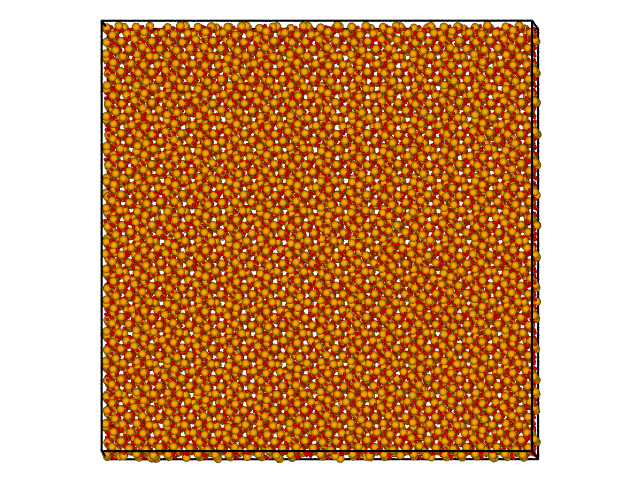
\includegraphics[width=0.24\textwidth]{graphics/initial_atoms.png}
    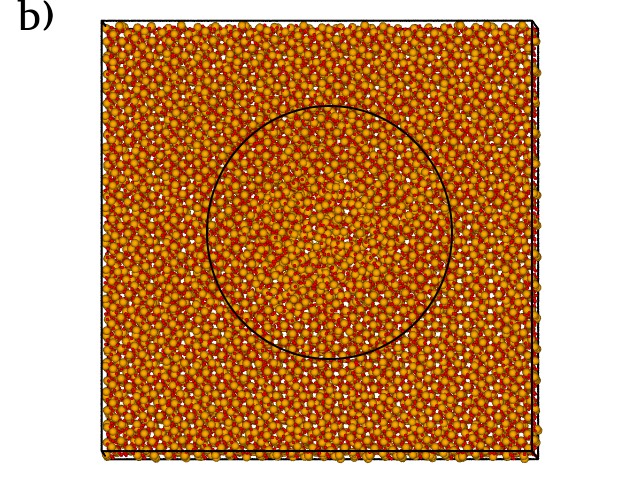
\includegraphics[width=0.24\textwidth]{graphics/spike_atoms.png}
    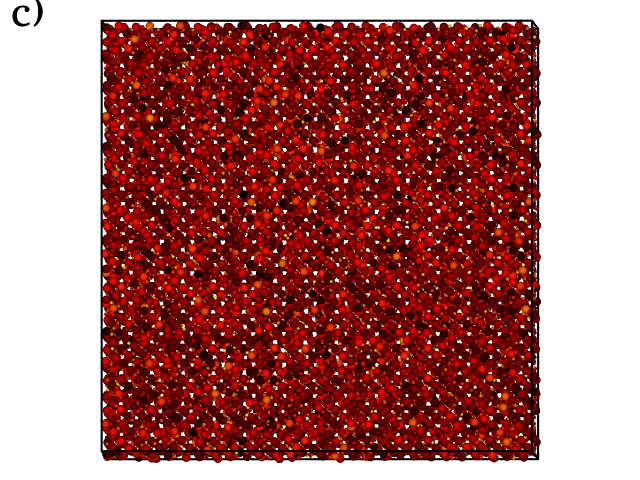
\includegraphics[width=0.24\textwidth]{graphics/initial.png}
    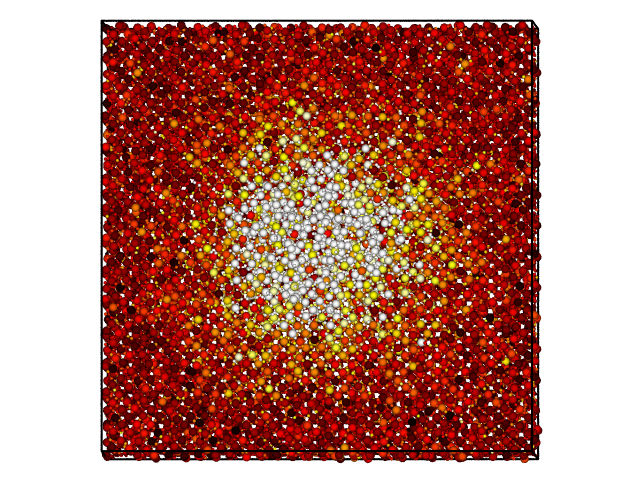
\includegraphics[width=0.24\textwidth]{graphics/spike.png}
  \end{center}
  \caption{Thermal Spike in SiO2}
\end{wrapfigure}

Previous studies have looked at the fine structure of SHI tracks (the narrow trails of permanent atomic distortion along penetrating SHI pathways) in thin film amorphous silica using small angle x-ray scattering (SAXS) measurements combine with non-equilibrium MD modeling and simulation techniques. These studies have successfully revealed that SHI tracks form a low density shell around the SHI path of penetration surrounded by an outer shell higher in density. The non-equlibrium MD calculations were carried out using an ~20k atom system where the track was produced by using the simple approach of instantaneous heating of  the atoms in the simulation cell along the SHI track path. This method has been motivated by the fact that most of the energy transfer from the electronic system to the atomic degrees of freedom occurs on the femtoseconds timescale.  The timescale of ionic displacements is much greater, implying the transfer is immediate. 

We intend to carry out similar simulations of comparable size that can be used to elucidate the structural changes observed in neutron scattering experiments of the average and local structure of these polymorphs of silica. Atomistic configurations from the end of this trajectory can then be fed into the RMC modeling to optimize the structure against the experimental data. The results of this study can help understand the fundamental degradation of silica materials exposed radiation damage and also to future work to manipulate nanoclusters within solid silica materials. 

An extension of this project would be to incorporate recently models that have been developed to address more realistic modeling of the electronic heat conduction to the atomic degrees of freedom. In these models, the solution of the electronic heat conduction is embedded into the MD simulations via including an electronic continuum used to solve a heat equation for modeling the energy transport between the atomic and electronic subsystems. The two-temperature model formalism of including the electron-phonon coupling has been previously used in modeling and simulating SHI bombardment of alpha-quartz, laser ablation, and shock simulations. Interestingly to our ICE-MAN project, this extension would allow us to bridge a quantum-to-molecular multiscale-modeling barrier. An important input parameter into the two-temperature model is the electronic specific heat. Recently, it has been shown that the electronic temperature depedence of the electronic specific heat can have an effect on the morphology of the SHI track that is formed.  To produce this relation, one calculates the difference in internal energy with change in the electronic temperature using finite-temperature density functional theory. Previous work of others have used the popular opEn Source Package for Research in Electronic Structure, Simulation, and Optimization (Quantum ESPRESSO) and the Vienna ab initio simulation package (VASP) softwares with proven scalability. Thus, we hope to use this project as a proof-of-concept workflow for ICE-MAN to: begin with quantum calculations, use outputs of these calculations as inputs into non-equilibrium MD simulations, and then use the atomic configurations of outputs from these simulations as inputs into RMC modeling to optimize the atomic structures against neutron scattering data.
